\chapter{Resultados y Discusión}

\section{Resultados}

\subsection{Análisis de complejidad}

La Tabla \ref{tab:complejidad} resume la complejidad derivada en el Capítulo 4 para cada algoritmo implementado. $n$ es el número de pedidos o puntos, $V$ y $E$ el número de lugares y arcos, $W$ la capacidad en décimas de kg, $R$ el número de repartidores, $K$ el tamaño máximo de zona, y $b$ y $d$ el grado medio y la longitud de los caminos explorados.

\begin{table}[h]
    \centering
    \caption{Complejidad Big-O de los algoritmos implementados.}
    \label{tab:complejidad}
    \small
    \begin{tabular}{llll}
        \toprule
        \textbf{Algoritmo} & \textbf{Paradigma} & \textbf{Tiempo} & \textbf{Espacio} \\
        \midrule
        Merge Sort                 & Divide y Vencerás & $\Theta(n\log n)$ & $O(n)$ \\
        Quick Sort                 & Divide y Vencerás & $O(n\log n)$ prom., $O(n^2)$ peor & $O(\log n)$ \\
        Búsqueda binaria           & Disminuir y Vencer & $O(\log n)$ & $O(1)$ \\
        Búsqueda por ID / sector   & Tabla hash        & $O(1)$ prom. & $O(n)$ \\
        Dijkstra desde cada lugar  & Greedy            & $O(V(V+E)\log V)$ & $O(V^2)$ \\
        Vecino más cercano         & Greedy            & $O(n^2)$ & $O(n)$ \\
        Asignación de emergencia   & Greedy            & $O(R)$ & $O(1)$ \\
        Partición en zonas de $K$  & Divide y Vencerás & $\Theta(n\log^2 n)$ & $O(n)$ \\
        Ruta por zonas de $K$      & DyV + Greedy      & $O(n^2/K)$ & $O(n)$ \\
        Partición en $R$ zonas     & Divide y Vencerás & $\Theta(n\log n\log R)$ & $O(n)$ \\
        Mochila 0/1                & Prog. Dinámica    & $O(N\cdot W)$ & $O(N\cdot W)$ \\
        Held-Karp (TSP)            & Prog. Dinámica    & $O(n^2 2^n)$ & $O(n\,2^n)$ \\
        Rutas simples              & Backtracking      & $O(b^d)$; peor $O(V\cdot V!)$ & $O(V)$ \\
        \bottomrule
    \end{tabular}
\end{table}

\subsection{Casos de prueba y resultados esperados}

La Tabla \ref{tab:casos} muestra los casos de prueba principales, con el resultado esperado calculado de forma independiente (a mano o por fuerza bruta) y el resultado obtenido. Todos forman parte de las 39 pruebas automáticas del Anexo C.

\begin{table}[h]
    \centering
    \caption{Casos de prueba con resultado esperado y obtenido.}
    \label{tab:casos}
    \footnotesize
    \begin{tabular}{p{2.9cm}p{4.3cm}p{4.3cm}c}
        \toprule
        \textbf{Algoritmo} & \textbf{Entrada} & \textbf{Esperado} & \textbf{Obtenido} \\
        \midrule
        Mochila 0/1 & pesos (1,2,3), valores (15,10,30), $W=4$ & valor 45 (ítems 1 y 3) & \checkmark \\
        Mochila 0/1 & 12 pedidos reales, $W=20$ kg & óptimo de los $2^{12}$ subconjuntos & \checkmark \\
        Mochila 0/1 & 15 pedidos reales, $W=5$ kg & carga $\le$ 5 kg (antes: 5.2 kg) & 4.2 kg \\
        Mochila voraz & pesos (1,2,3), $W=4$ & valor 25 (subóptimo) & \checkmark \\
        Held-Karp & matriz asimétrica $3\times3$ & 0$\to$2$\to$1$\to$0, 20 m & \checkmark \\
        Held-Karp por zona & 8 pedidos reales & distancia $\le$ Greedy & \checkmark \\
        Backtracking & diamante, sin cierres & 2 rutas; óptima por N03 (5 m) & \checkmark \\
        Backtracking & diamante, N01--N03 cerrada & 1 ruta, por N02 & \checkmark \\
        Backtracking & San Blas $\to$ Wanchaq & 27 rutas; óptima 1,778.62 m & \checkmark \\
        Backtracking con poda & San Blas $\to$ Wanchaq & misma óptima, menos estados & 20 vs 146 \\
        D\&C en $R$ zonas & 6 pedidos, $R=1..4$ & $R$ zonas, tamaños $\pm1$ & \checkmark \\
        D\&C por repartidor & 30 pedidos, 3 repartidores & 3 zonas, 1 por repartidor & \checkmark \\
        Greedy emergencia & pedido urgente, 3 repartidores & el más cercano con capacidad & \checkmark \\
        Búsqueda binaria & ID existente / inexistente & índice / $-1$ & \checkmark \\
        \bottomrule
    \end{tabular}
\end{table}

\subsection{Ordenación}

Con 10, 20 y 30 pedidos, Merge Sort tardó 0.011, 0.023 y 0.059 ms, y Quick Sort 0.010, 0.022 y 0.032 ms (promedio de 20 repeticiones). Con tamaños tan pequeños ambos son prácticamente instantáneos; Quick Sort resulta algo más rápido por trabajar en el mismo arreglo, mientras que Merge Sort conserva el orden relativo de los empates (es estable), lo que mantiene el orden de llegada entre pedidos de igual prioridad.

\subsection{Greedy frente a Held-Karp: tiempo}

\begin{table}[h]
    \centering
    \caption{Tiempo de ejecución (ms): Greedy frente a Held-Karp.}
    \label{tab:benchmark}
    \begin{tabular}{cccc}
        \toprule
        $n$ & \textbf{Greedy (ms)} & \textbf{Held-Karp (ms)} & \textbf{Held-Karp / Greedy} \\
        \midrule
        3  & 0.041 & 0.027  & $0.7\times$ \\
        5  & 0.007 & 0.059  & $8.4\times$ \\
        8  & 0.013 & 0.929  & $71.5\times$ \\
        10 & 0.014 & 7.689  & $549\times$ \\
        12 & 0.017 & 22.166 & $1{,}304\times$ \\
        \bottomrule
    \end{tabular}
\end{table}

La Tabla \ref{tab:benchmark} y la Figura \ref{fig:tiempo_vs_n} muestran que el tiempo de Held-Karp crece exponencialmente, mientras que el del Greedy apenas varía. Con $n\le 5$ ambos tiempos son de microsegundos y están dominados por el costo fijo de llamar a una función en Python, por lo que la relación entre ellos no es significativa.

\begin{figure}[h]
    \centering
    \caption[Tiempo de ejecución Greedy vs Held-Karp]
    {Tiempo medido (ms, escala logarítmica) en función de $n$. Las líneas punteadas son las curvas teóricas $O(n^2)$ y $O(n^2 2^n)$ escaladas al primer punto.}
    \label{fig:tiempo_vs_n}
    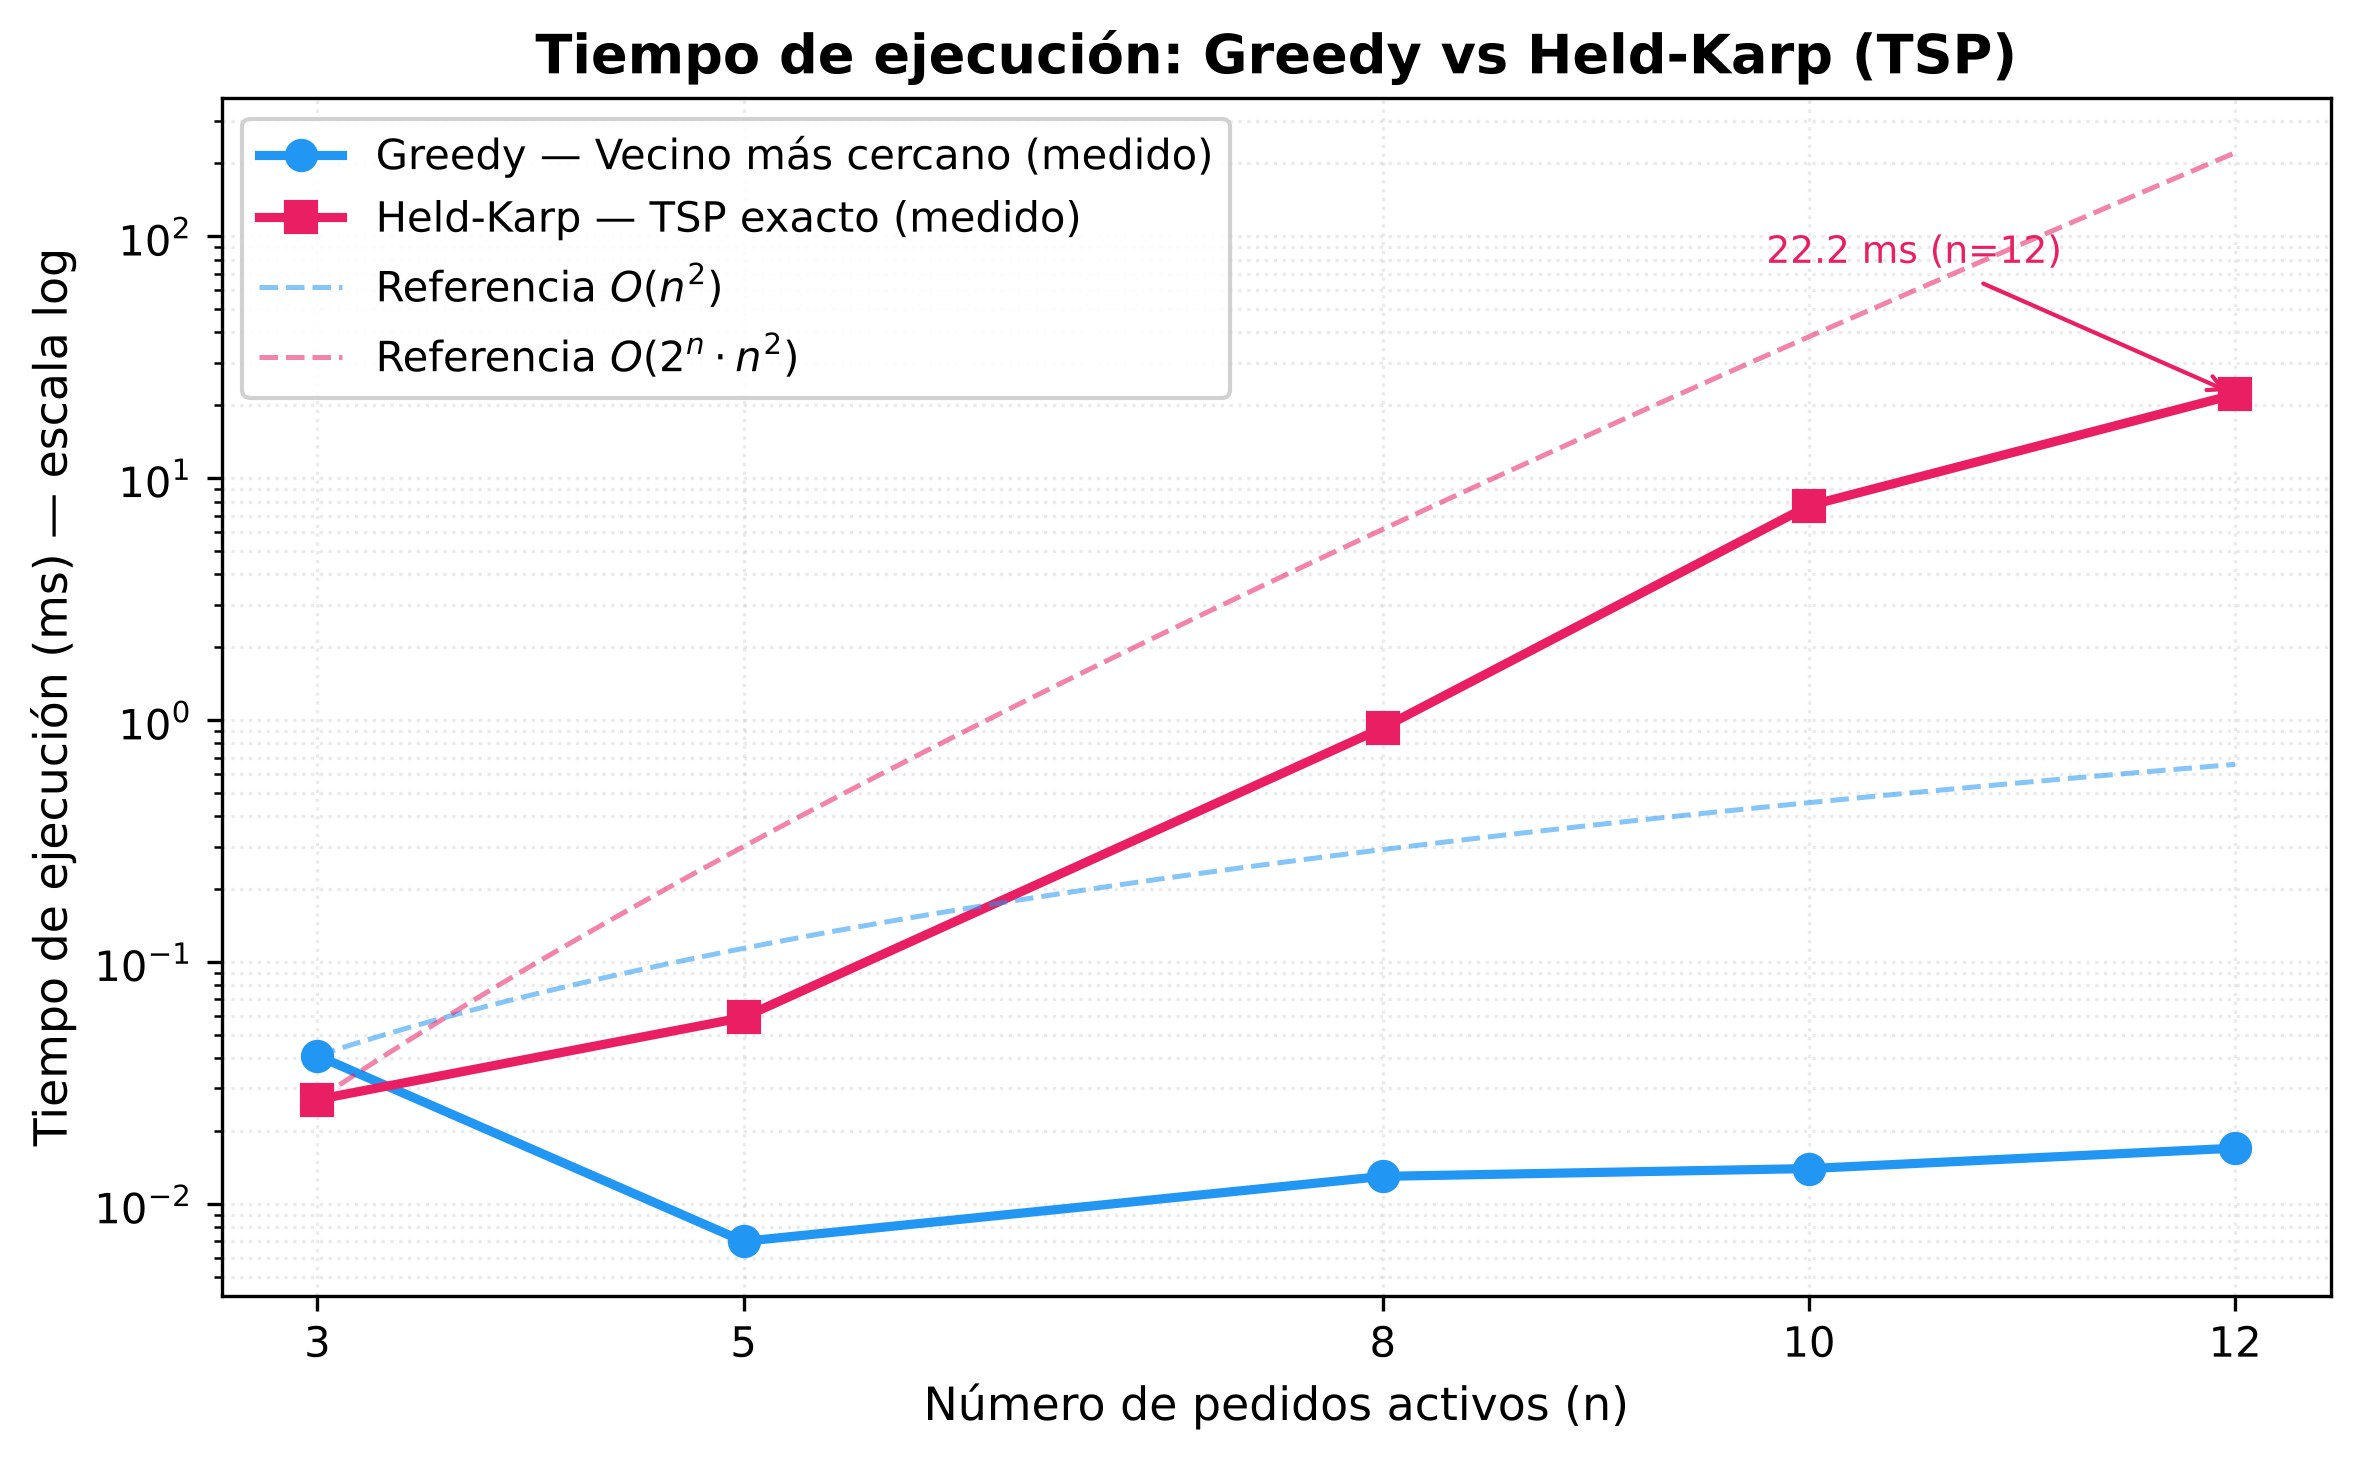
\includegraphics[width=135mm]{figuras/fig1_tiempo_vs_n.png}
\end{figure}

\subsection{Greedy frente a Held-Karp: calidad}

\begin{table}[h]
    \centering
    \caption{Distancia total del recorrido (m) y exceso del Greedy sobre el óptimo.}
    \label{tab:calidad}
    \begin{tabular}{cccc}
        \toprule
        $n$ & \textbf{Held-Karp (m)} & \textbf{Greedy (m)} & \textbf{Exceso (\%)} \\
        \midrule
        3  & 1{,}866.35  & 1{,}866.35  & 0.00  \\
        5  & 3{,}685.04  & 3{,}685.04  & 0.00  \\
        8  & 7{,}608.16  & 9{,}474.50  & 24.53 \\
        10 & 8{,}790.04  & 10{,}656.39 & 21.23 \\
        12 & 11{,}785.27 & 13{,}651.62 & 15.84 \\
        \bottomrule
    \end{tabular}
\end{table}

\begin{figure}[h]
    \centering
    \caption[Calidad de ruta: Greedy vs Held-Karp]
    {Izquierda: distancia total del recorrido (km). Derecha: exceso porcentual del Greedy sobre el óptimo.}
    \label{fig:calidad_ruta}
    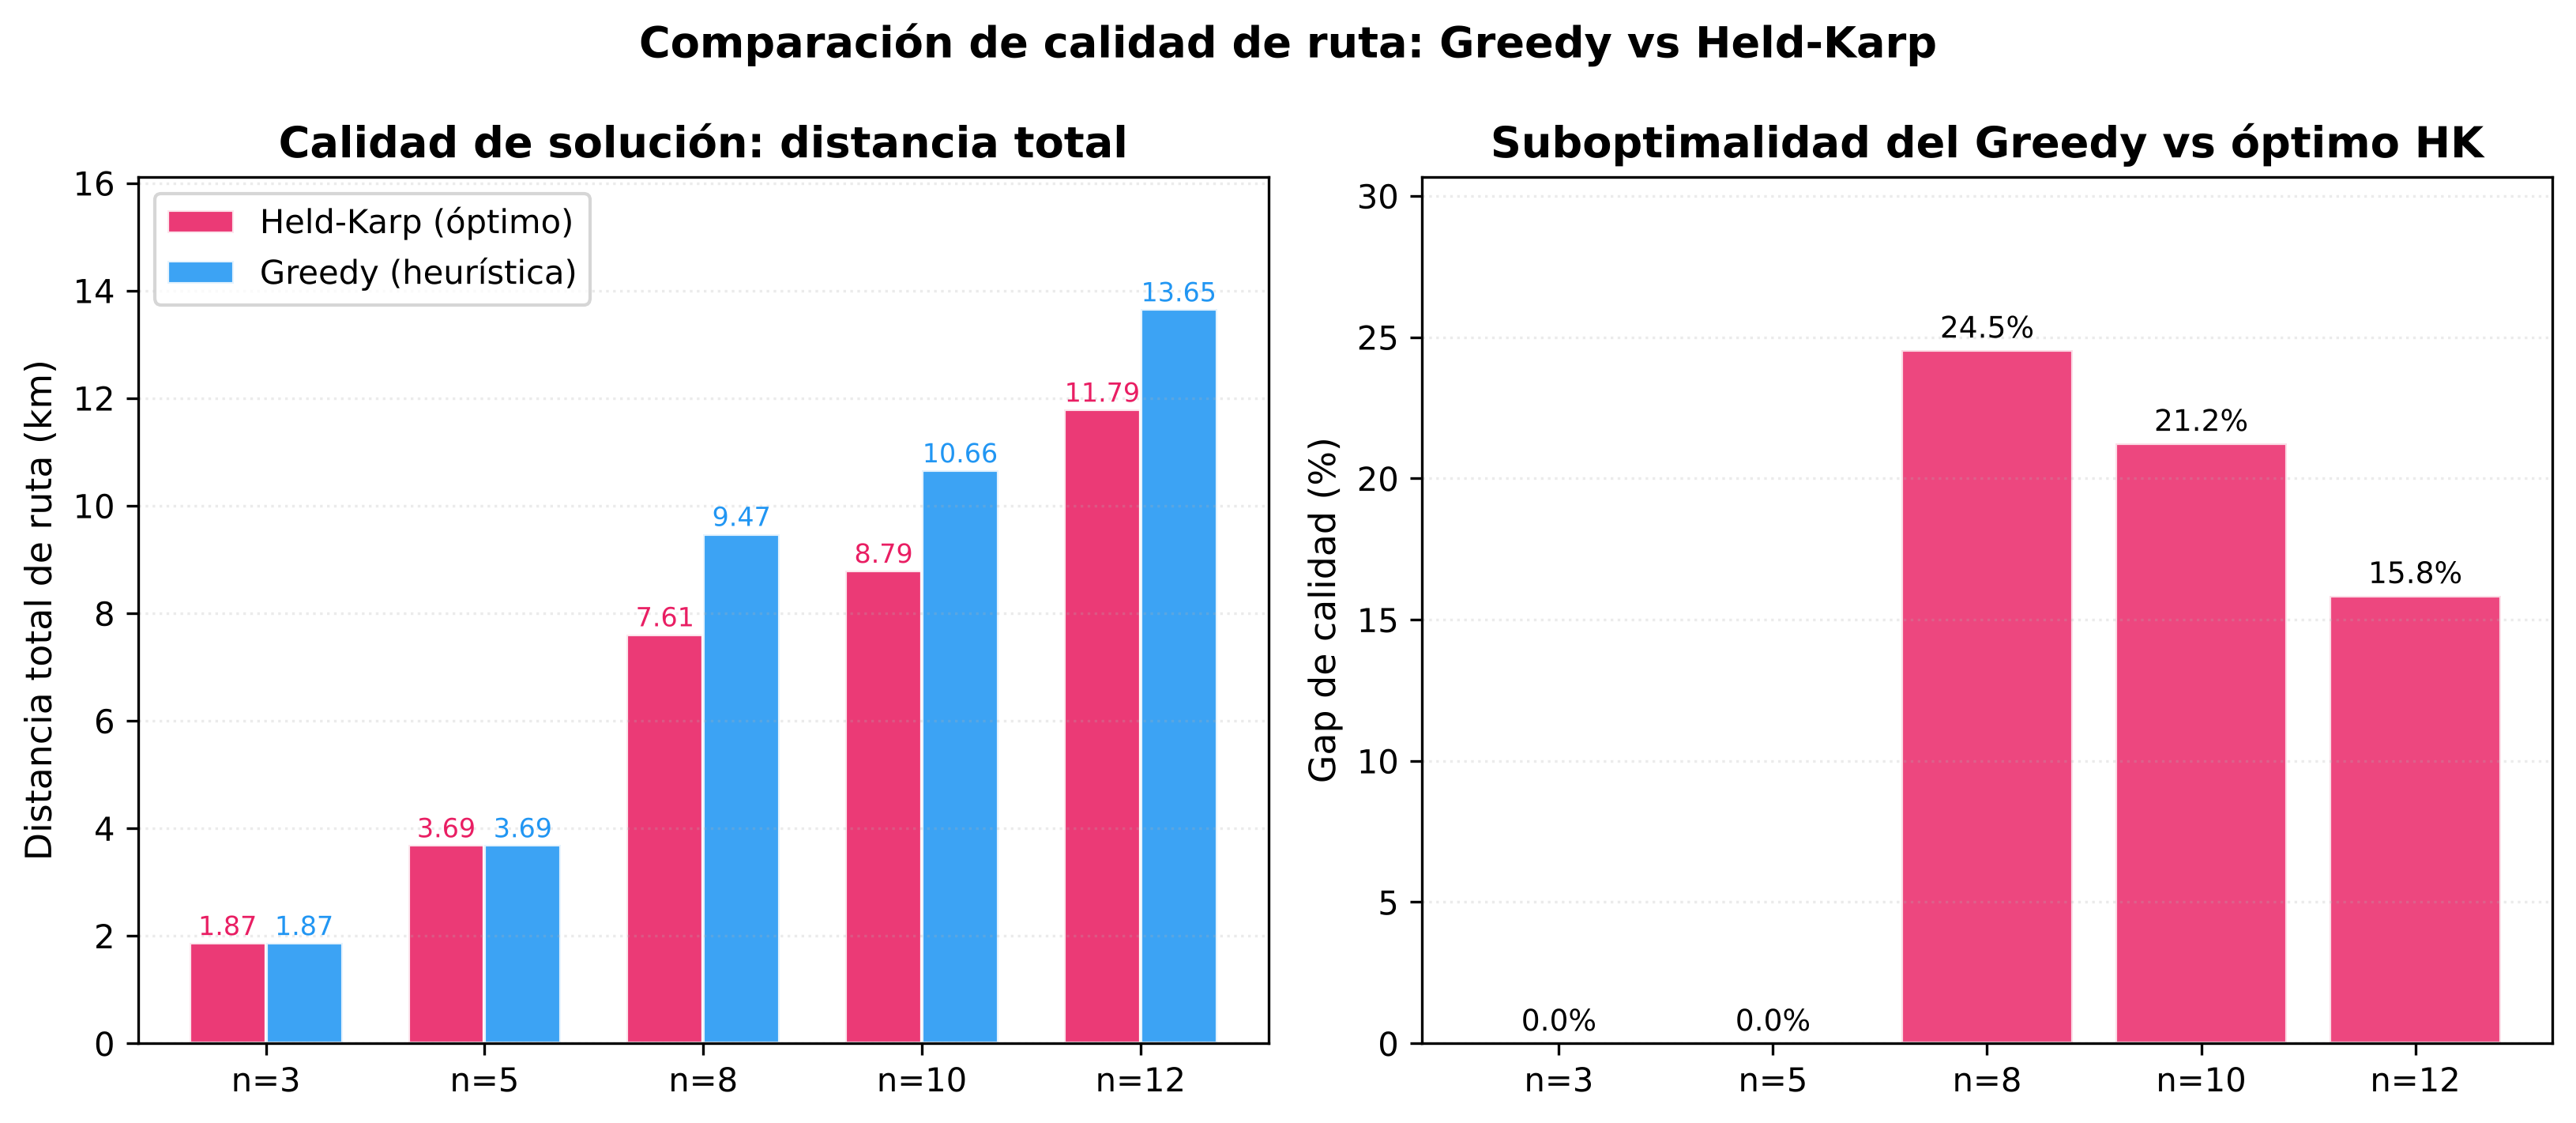
\includegraphics[width=145mm]{figuras/fig2_calidad_ruta.png}
\end{figure}

\subsection{Backtracking: todas las rutas y efecto de la poda}

En el caso del enunciado, de San Blas (N02) a Wanchaq (N11) con todas las calles abiertas, la búsqueda exhaustiva encontró \textbf{27 rutas simples}, de 1,778.62 m a 35,284.11 m. La más corta es N02$\to$N08$\to$N10$\to$N11 (1,778.62 m); la segunda, N02$\to$N09$\to$N11, mide solo 12.55 m más. Al cerrar por mantenimiento la calle San Blas--Limacpampa (N02--N08), quedan 25 rutas y el algoritmo elige N02$\to$N09$\to$N11 (1,791.17 m), sin pasar nunca por la calle cerrada.

\begin{table}[h]
    \centering
    \caption{Backtracking sin poda (exhaustivo) y con poda en cuatro pares origen--destino.}
    \label{tab:backtracking}
    \small
    \begin{tabular}{lccccccc}
        \toprule
        & \multicolumn{3}{c}{\textbf{Sin poda}} & \multicolumn{3}{c}{\textbf{Con poda}} & \\
        \cmidrule(lr){2-4}\cmidrule(lr){5-7}
        \textbf{Par} & \textbf{Rutas} & \textbf{Estados} & \textbf{ms} & \textbf{Rutas} & \textbf{Estados} & \textbf{ms} & \textbf{Óptima (m)} \\
        \midrule
        N01$\to$N04 & 1   & 776   & 0.71 & 1 & 448 & 0.41 & 790.80 \\
        N02$\to$N11 & 27  & 146   & 0.19 & 1 & 20  & 0.02 & 1{,}778.62 \\
        N01$\to$N15 & 152 & 775   & 0.92 & 2 & 142 & 0.18 & 4{,}524.34 \\
        N05$\to$N19 & 500$^{*}$ & 3{,}129 & 4.09 & 7 & 955 & 0.73 & 9{,}034.33 \\
        \bottomrule
        \multicolumn{8}{l}{\footnotesize $^{*}$ Alcanzó el tope de seguridad de 500 rutas; con poda se obtuvo la misma óptima.}
    \end{tabular}
\end{table}

La Tabla \ref{tab:backtracking} y la Figura \ref{fig:backtracking} comparan ambos modos. En los cuatro pares la ruta óptima con poda coincide con la del modo exhaustivo, como garantiza el argumento del Capítulo 4, y los estados visitados se reducen entre 42\% y 86\%. Con poda, la columna \emph{Rutas} cuenta solo las rutas que fueron mejorando la mejor distancia conocida: por eso, si se necesita la lista completa de alternativas (por ejemplo, para ofrecer una ruta de reserva), la poda debe desactivarse. El par N01$\to$N04 muestra que el número de estados no depende solo del número de rutas: hay una única ruta simple, pero la red dirigida obliga a explorar 776 estados en callejones sin salida.

\begin{figure}[h]
    \centering
    \caption[Backtracking con y sin poda]
    {Estados visitados (izquierda) y rutas registradas (derecha) por el Backtracking sin poda y con poda.}
    \label{fig:backtracking}
    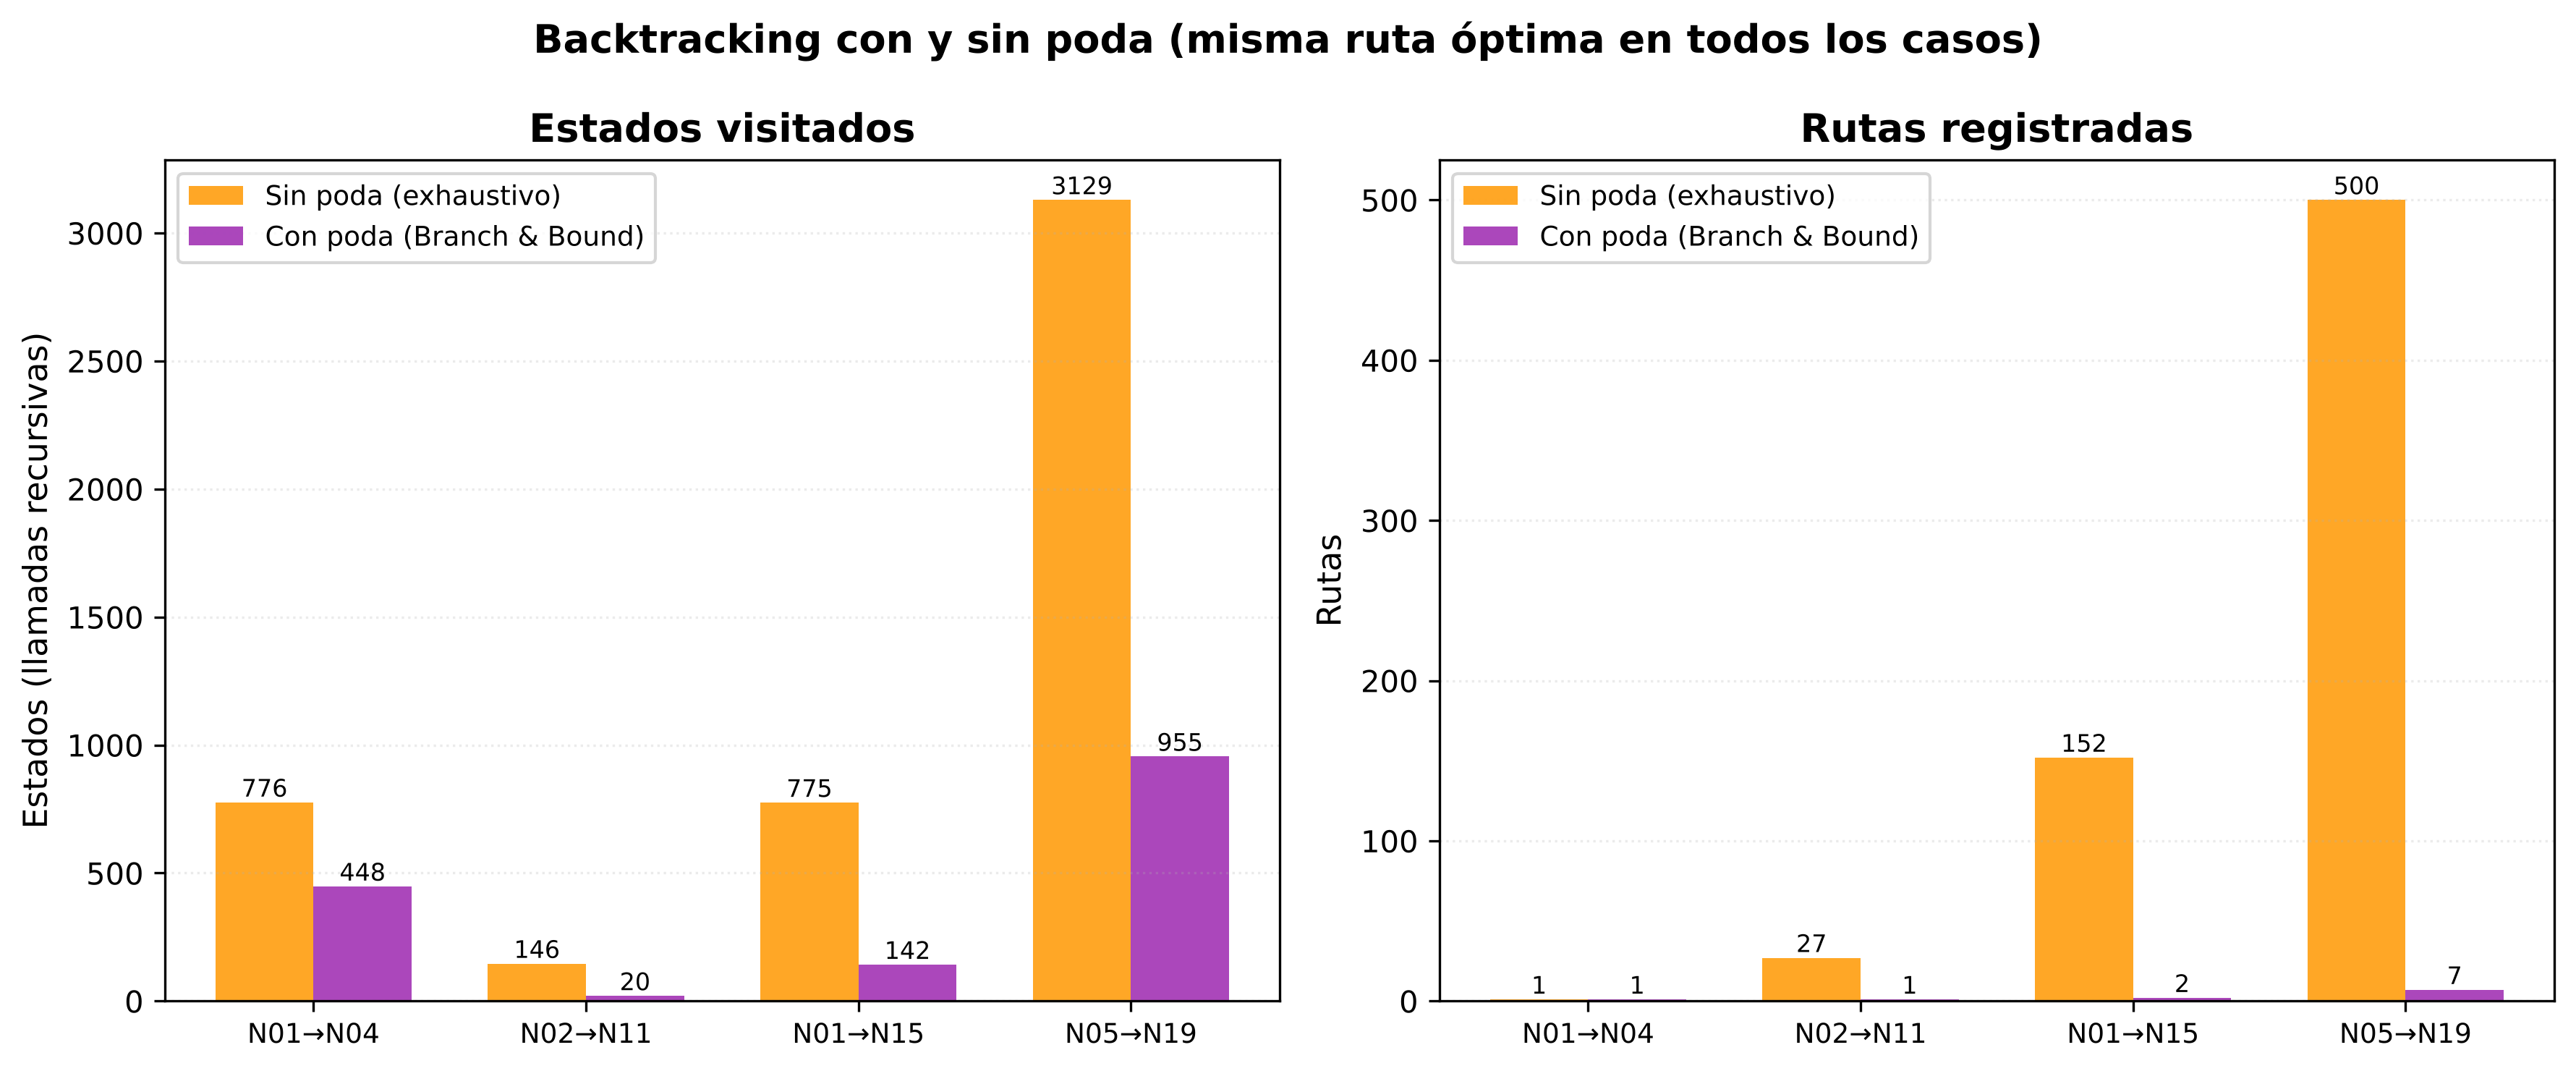
\includegraphics[width=145mm]{figuras/fig3_backtracking.png}
\end{figure}

\subsection{Mochila 0/1: Programación Dinámica frente a Greedy}

Con capacidad de 25 kg, la Mochila por PD obtuvo un valor mayor o igual al de la heurística voraz por valor/kg en todos los casos (Tabla \ref{tab:mochila}): igual con $N=5$, 10, 25 y 30, y superior con $N=15$ (S/.~1,640 frente a S/.~1,625) y $N=20$ (S/.~1,700 frente a S/.~1,695). La tabla de PD llegó a 7,781 celdas y su cálculo nunca superó 0.7 ms.

\begin{table}[h]
    \centering
    \caption{Valor cargado (S/.) con capacidad de 25 kg.}
    \label{tab:mochila}
    \begin{tabular}{cccccc}
        \toprule
        $N$ & \textbf{PD} & \textbf{Voraz} & \textbf{Celdas de la tabla} & \textbf{PD (ms)} & \textbf{Voraz (ms)} \\
        \midrule
        5  & 685   & 685   & 1{,}506 & 0.131 & 0.017 \\
        10 & 1{,}215 & 1{,}215 & 2{,}761 & 0.233 & 0.018 \\
        15 & 1{,}640 & 1{,}625 & 4{,}016 & 0.306 & 0.026 \\
        20 & 1{,}700 & 1{,}695 & 5{,}271 & 0.427 & 0.037 \\
        25 & 1{,}930 & 1{,}930 & 6{,}526 & 0.492 & 0.043 \\
        30 & 2{,}365 & 2{,}365 & 7{,}781 & 0.602 & 0.058 \\
        \bottomrule
    \end{tabular}
\end{table}

Durante la revisión se detectó y corrigió un error en la discretización de pesos: la versión inicial redondeaba cada peso al kilogramo más cercano (2.2 kg contaba como 2 kg y 4.5 kg como 4 kg), y con los 15 primeros pedidos llegó a elegir 5.2 kg para una capacidad de 5 kg y 15.2 kg para una de 15 kg. La versión final trabaja con precisión de 0.1 kg, redondea los pesos hacia arriba y la capacidad hacia abajo, y una prueba automática verifica que la carga nunca exceda la capacidad.

\subsection{Divide y Vencerás}

\textbf{Una zona por repartidor.} Con los 30 pedidos y los 3 repartidores, la partición produjo tres zonas de 10 pedidos y cada repartidor calculó con Held-Karp la ruta óptima de su zona (Tabla \ref{tab:zonas}). Entre los tres recorren 30.22 km, frente a 43.35 km de un único repartidor que atiende todo con el Greedy; además trabajan en paralelo, por lo que el reparto termina cuando acaba la ruta más larga (12.46 km).

\begin{table}[h]
    \centering
    \caption{Divide y Vencerás: una zona por repartidor (30 pedidos).}
    \label{tab:zonas}
    \begin{tabular}{llcc}
        \toprule
        \textbf{Zona} & \textbf{Repartidor} & \textbf{Pedidos} & \textbf{Ruta óptima (m)} \\
        \midrule
        1 & REP-03 (furgoneta, Marcavalle)       & 10 & 12{,}457.73 \\
        2 & REP-01 (bicicleta, Plaza de Armas)   & 10 & 11{,}974.11 \\
        3 & REP-02 (motocicleta, Av. El Sol)     & 10 & 5{,}788.10 \\
        \midrule
        \multicolumn{3}{l}{Total del equipo} & 30{,}219.94 \\
        \multicolumn{3}{l}{Un solo repartidor (Greedy, desde la Plaza de Armas)} & 43{,}352.76 \\
        \bottomrule
    \end{tabular}
\end{table}

\textbf{Un repartidor y zonas de $K$ pedidos.} Con pedidos sintéticos (Figura \ref{fig:mochila_dyv}, derecha, y Anexo E), el tiempo de Divide y Vencerás con $K=5$ pasó de 0.22 ms ($n=30$) a 11.6 ms ($n=480$), similar al del Greedy global. Sin embargo, su ruta fue más larga para $n\ge60$: como los pedidos se concentran en solo 20 lugares, el corte por coordenadas separa en zonas distintas pedidos de un mismo lugar y obliga a volver a él, mientras que el Greedy los atiende todos de una vez. Para un único repartidor, la segmentación sirve para organizar el trabajo, no para acortar la ruta; su ventaja aparece al repartir zonas entre varios repartidores.

\begin{figure}[h]
    \centering
    \caption[Mochila y Divide y Vencerás]
    {Izquierda: valor cargado por la Mochila con PD y por la heurística voraz. Derecha: rutas de las tres zonas frente a un único repartidor voraz.}
    \label{fig:mochila_dyv}
    \includegraphics[width=145mm]{figuras/fig4_mochila_dyv.png}
\end{figure}

\subsection{Verificación de correctitud y estabilidad}

Las 39 pruebas unitarias de \texttt{tests/} se aprobaron sin fallos (Anexo C). La prueba automática de la interfaz ejecutó todas las funcionalidades de las siete pestañas, incluido el \textit{benchmark} en vivo, sin errores ni bloqueos; las capturas del Anexo D proceden de esa ejecución.

\section{Discusión: ¿cuándo usar cada enfoque?}

\textbf{Greedy frente a Programación Dinámica en rutas.} Held-Karp garantiza el recorrido óptimo, pero por su costo $O(n^2 2^n)$ su tiempo se multiplicó por 376 entre $n=5$ y $n=12$, hasta 22 ms; el Greedy respondió siempre en menos de 0.05 ms, pero produjo recorridos hasta 24.5\% más largos. Por tanto, conviene PD cuando el número de paradas es pequeño ($n \le 12$--14) y el ahorro de distancia importa, por ejemplo en la ruta del día de cada repartidor o dentro de cada zona de Divide y Vencerás. Conviene el Greedy cuando hay muchas paradas, cuando la respuesta debe ser inmediata (pedidos de emergencia) o cuando la ruta se recalcula continuamente.

\textbf{Greedy frente a Programación Dinámica en la carga.} En la mochila la PD resulta casi siempre preferible: su costo $O(N\cdot W)$ es pseudo-polinomial y, con capacidades reales de vehículos, la tabla tiene unos pocos miles de celdas y se calcula en menos de 1 ms. La heurística voraz solo tendría sentido con capacidades enormes o precisión muy fina, donde $W$ haría crecer demasiado la tabla.

\textbf{Backtracking.} Es el único enfoque que enumera \emph{todas} las alternativas y admite cualquier restricción (calles cerradas, sentidos, tramos obligatorios). Su costo es exponencial: en la red de 20 lugares se mantiene por debajo de 5 ms, pero el par N05$\to$N19 ya supera las 500 rutas simples. Conviene cuando el grafo es pequeño o la zona de búsqueda está acotada, cuando se necesitan rutas de reserva, o con la poda activada cuando solo interesa la ruta óptima bajo restricciones.

\textbf{Divide y Vencerás.} Su aporte es dividir el trabajo: al asignar una zona a cada repartidor, cada subproblema queda lo bastante pequeño para resolverse de forma exacta, y el equipo recorre 30\% menos distancia que un único repartidor. Para un solo vehículo no mejora la calidad de la ruta.

En conjunto, los paradigmas no compiten sino que se complementan. El sistema combina Divide y Vencerás para repartir zonas, PD para cargar cada vehículo y ordenar cada zona, Greedy para las decisiones urgentes y Backtracking cuando las restricciones de la red vial obligan a buscar alternativas.
